\documentclass[border=2pt]{standalone}
\usepackage{tikz}
\begin{document}
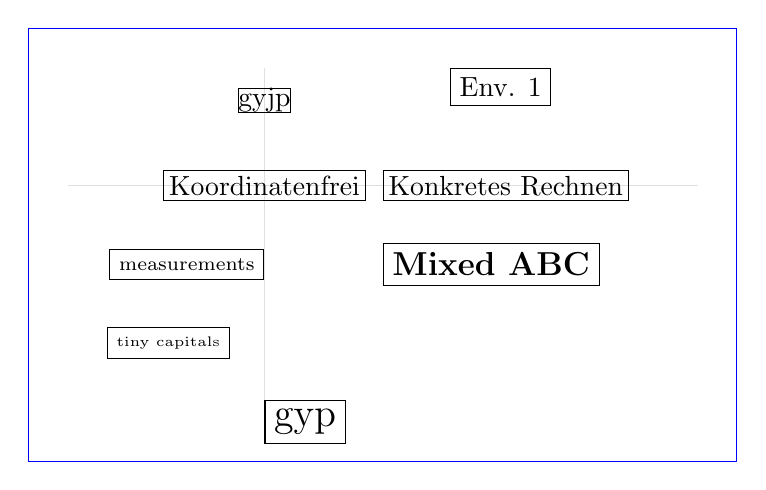
\begin{tikzpicture}
  \draw[blue] (-3,-3.5) rectangle (6,2);
  \draw[gray!25] (-2.5,0) -- (5.5,0) (0,-3) -- (0,1.5);
  \node[draw,inner sep=2pt] (a) at (0,0) {Koordinatenfrei};
  \node[draw,inner sep=2pt,anchor=west] (b) at (1.5,0) {Konkretes Rechnen};
  \node[draw,inner sep=0pt,anchor=base] at (0,1) {gyjp};
  \node[draw,anchor=north] at (3,1.5) {Env. 1};
  \node[draw,font=\scriptsize,anchor=east] at (0,-1) {measurements};
  \node[draw,font=\large\bfseries,anchor=west] at (1.5,-1) {Mixed ABC};
  \node[draw,font=\tiny,anchor=west] at (-2,-2) {tiny capitals};
  \node[draw,font=\Large,anchor=west] at (0,-3) {gyp};
\end{tikzpicture}
\end{document}
